\documentclass{article}
\usepackage{fontspec}
\usepackage{amsmath}
\usepackage{amssymb}
\usepackage{xcolor}
\usepackage{soul}
\usepackage{array}
\usepackage{float}
\usepackage{tikz}
\usepackage[framemethod=tikz]{mdframed}
\usetikzlibrary{shadows}
\usepackage{graphicx}
\usepackage{hyperref}[colorlinks=true]
\usepackage{geometry}[margin=0.5in]
\usepackage{polynom}
\sethlcolor{yellow}
\setmainfont{Times New Roman}

\setlength{\parindent}{0cm}

\definecolor{darkgreen}{RGB}{39, 145, 45}

\newcounter{question}[section]
\renewcommand{\thequestion}{\thesection .\arabic{question}.}
\newcommand{\question}[1]{\par\stepcounter{question}\hl{\bf\thequestion} \quad #1 \par}

\newcounter{subquestion}[question]
\renewcommand{\thesubquestion}{\alph{subquestion}}
\newcommand{\subquestion}[1]{\stepcounter{subquestion}\textbf{(\thesubquestion)}\space \emph{#1}\par}

\newcommand{\substep}[1]{{\par\large\em\textbf{\rightarrow}\space #1 \par}\vspace{0.1cm}}

\newcommand{\solnstitle}{\vspace{0.2cm}
{\bf\large\centering\color{red} \thequestion\space Solutions \par}}
\newenvironment{solnstable}{
    \begin{table}[H]
        \renewcommand{\arraystretch}{1.5}
        \color{red}
        \begin{tabular}{l|m{4cm}}
}{
        \end{tabular}
    \end{table}
}
\newenvironment{solns}{
    \solnstitle
    
}{
        
}
\newcounter{step}[subquestion]
\renewcommand{\thestep}{Step \Roman{step}}
\newcommand{\step}[1]{\par\vspace{0.1cm}{\centering\bf \stepcounter{step}\thestep :\space#1 \par}}

\newenvironment{answer}{}{}
\surroundwithmdframed[
    linewidth=1pt,
    linecolor=red,
    frametitle={\color{red}Final Answer}, 
    frametitlealignment=\centering
]{answer}

\newenvironment{knowledge}{
    \begin{enumerate}
}{
    \end{enumerate}
}
\surroundwithmdframed[
    linewidth=1pt,
    linecolor=darkgreen,
    frametitle={\color{darkgreen}Required Knwoledge}, 
    frametitlealignment=\centering
]{knowledge}

\newenvironment{checkanswer}{}{
    \par\checkmark\space The solution has been verified and is correct.
}
\surroundwithmdframed[
    linecolor=orange,
    linewidth=3pt,
    roundcorner=10pt,
    frametitle={Checking Your Answer},
    frametitlealignment=\centering,
    shadow=true,
    shadowcolor=yellow
]{checkanswer}

\newcommand{\TRUE}{\textbf{\sffamily\textcolor{darkgreen}{TRUE}\space}}
\newcommand{\FALSE}{\textbf{\sffamily\textcolor{red}{FALSE}\space}}

% \newcommand{\checkmark}{\tikz\fill[scale=0.4](0,.35) -- (.25,0) -- (1,.7) -- (.25,.15) -- cycle;}

\catcode`?=11 % Some commands use question marks in their names
\newcommand{\geq?}{\stackrel{?}{\geq}}

\newmdenv[
    linewidth=5pt,
    linecolor=red,
    frametitle={\Huge Disclaimer},
    frametitlealignment=\centering,
    backgroundcolor=red!10
]{disclaimer}
\begin{document}
    {
        \centering
        \Huge{Exam Practice \par}
        \vspace{0.5cm}
        \large{A comprehensive set of practice questions on all topics covered on the final exam \par}
        \vspace{0.5cm}
        {Version 1 \par}
        \vspace{0.5cm}
        {\small By Edouard Des Parois Perrault \par}
    }
    \begin{disclaimer}
        The problems within this document are heavily inspired off of the math textbook as well as those that were given in class.
    \end{disclaimer}
    \tableofcontents
    \section{Remainder Theorem}
    \question{$2x^n + ax^2 - 6$ leaves a remainder of $-7$ when it is divided by $x-1$. It also leaves a remainder of 129 when divided by $x-3$. What is $a$ and $n$ given that $n \in \mathbb{N}$}
    \begin{knowledge}
        \item Factor Theorem
        \item Basic algebra ($2 \cdot 1^n = 2$)
    \end{knowledge}
    \begin{solns}
        \step{Soving for $a$}
        \begin{solnstable}
            $f(1)=-7$ & By the remainder theorem \\
            $2(1)^n + a - 6 = -7$ & Plug in the $1$. \\
            $2 + a - 6 = -7$ & $2\cdot 1^n = 2$ \\
            $a = -3$ & Solve for $a$.
        \end{solnstable}
        \step{Solving for $n$}
        \begin{solnstable}
            $f(-3) = 129$ & By the remainder theorem\\
            $2(-3)^n + (-3)(-3)^2 - 6 = 129$ & Plug in $-3$ \\
            $(-3)^n = 81$ & Simplify \\
            $n = 4$ & No need for logs for this particular exponent problem.
        \end{solnstable}
        \begin{answer}
            $n = 4$ \\
            $a = -3$
        \end{answer}
    \end{solns}
    \section{Polynomial Rules}
    \question{A polynomial has
    \begin{enumerate}
        \item A degree of 5
        \item A leading coefficient of 2
        \item $x^4$ has a coefficient of 3.
        \item The $y-$intercept is 5.
        \item Its only two real zeroes are $\frac{1}{2}$ and $1 \pm \sqrt{2}$.
        \item Its other roots are $m \pm ni$, $n > 0$.
    \end{enumerate}
    What is $m$ and $n$?}
    \begin{knowledge}
        \item Sum of roots
        \item Product of roots
    \end{knowledge}
    \begin{solns}
        \step{Sum of Roots}
        \begin{solnstable}
            $\Sigma = \frac{-a_{n-1}}{a_n}$ & Using sum of roots \\
            $\frac{-3}{2}$ & \\
            $0.5 + 1 + \sqrt{2} + 1 - \sqrt{2} + m + ni + m - ni = \frac{-3}{2}$ & Equate to the actual sum of roots to solve. \\
            $2.5 + 2m = \frac{-3}{2}$ & \\
            $2m = -4$ & \\
            $m = -2$ & Solve for $m$ \\
        \end{solnstable}
        \step{Product of Roots}
        \begin{solnstable}
            $\Pi = \frac{(-1)^n a_0}{a_n}$ & Using the product of roots formula\\
            $\Pi = \frac{-5}{2}$ & \\
            $\left(\frac{1}{2}\right)(1+\sqrt{2})(1-\sqrt{2})(m-ni)(m+ni) = \frac{-5}{2}$ & Equate the product of roots to the formula \\
            $\left(\frac{1}{2}\right)(1-2)(m^2 - (ni)^2) = \frac{-5}{2}$ & \\
            $\left(\frac{-1}{2}\right)(m^2 + n^2) = \frac{-5}{2}$ & Simplify \\
            $-(4+n^2) = \frac{-5}{2}$ & Plug in the value of $m$ determined earlier. \\
            $-4-n^2 = -5$ & \\
            $-n^2 = -1$ & \\
            $n = \pm 1$ & \\
            $n = 1$ & $n < 0$ because of the question \\
        \end{solnstable}
        \begin{answer}
            $m = -2$ \\
            $n = 1$
        \end{answer}
    \end{solns}
    \question{Find all values of the real parameter $m$, $m \neq 0$, for which the equation $(mx)^2 + 3mx + 1 - m = 0$ has no solutions.}
    \begin{knowledge}
        \item Calculating the discriminate 
        \item Quadratic inequalities ($\Delta < 0$)
    \end{knowledge}
    \begin{solns}
        \step{Stating what is known}
        \begin{solnstable}
            $(mx)^2 + 3mx + 1 - m = 0$ & \\
            $m^2x^2 + 3mx +1 -m = 0$ & \\
            $ax^2 + bx +c$ & \\
            $a = m^2$ & \\
            $b = 3m$ & \\
            $c = 1 - m$ &\\
        \end{solnstable}
        \step{Find when $\Delta = 0$}
        \begin{solnstable}
            $\Delta = 0$ & \\
            $b^2 - 4ac = 0$ & Expand $\Delta$\\
            $(3m)^2 - 4m^2(1-m) = 0$ & Plug in $a$, $b$, and $c$. \\
            $3^2 m^2 -4m^2 +4 m^3 = 0$ & \\
            $4m^3 + 5m^2 = 0$ &  \\
            $m^2(4m+5) = 0$ & Simplify\\
            $m \in \{ 0, \frac{-5}{4} \}$ & Solve for roots by factoring \\
        \end{solnstable}
        \step{Find when $\Delta < 0$}
        \noindent This is done using graphical analysis, as shown below using Geogebra. A sketch of the function on a number line is also possible. The idea is to see when it is below the x-axis.
        \begin{figure}[H]
            \centering
            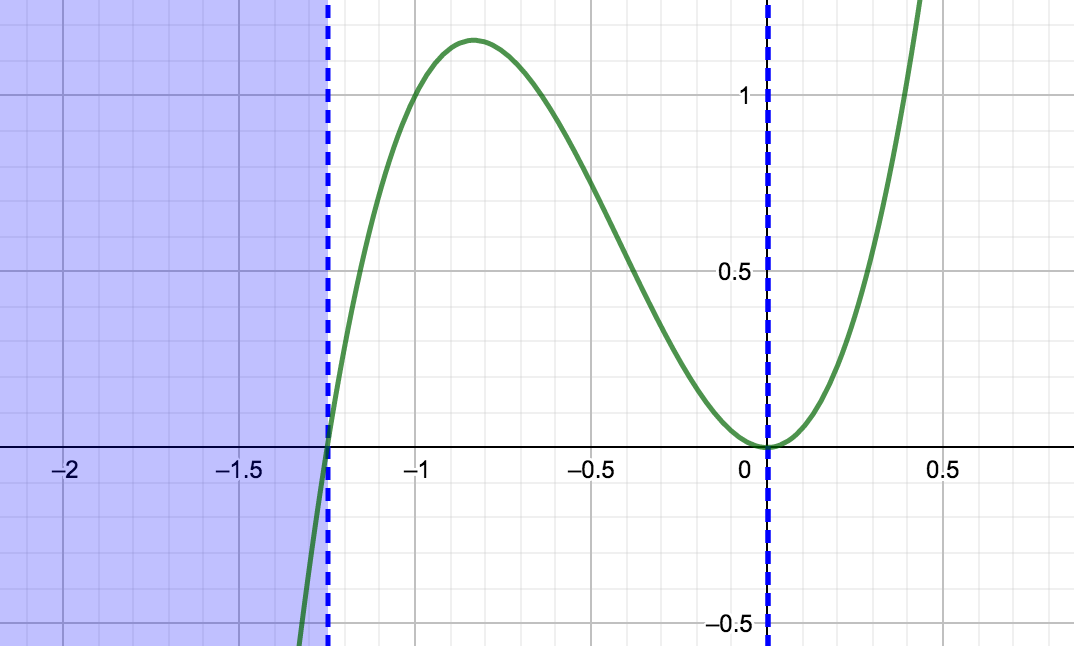
\includegraphics[scale=0.5]{Images/delta-mx2.png}
            \caption{Graphical analysis}
        \end{figure}
        \begin{answer}
            $m < \frac{-5}{4}$. This means that whenever $m$ is less than and \textbf{not} equal to $\frac{-5}{4}$, the function has no real roots. Note that the quadratic function mapping $\Delta$ and the function itself are completely separate.
        \end{answer}
    \end{solns}
    \newcommand{\questionpolynomial}{-3x^5 - x^4 + 5x^3 + 9x^2 - 11x + 20 = 0}
    \question{Given the polynomial $\questionpolynomial$, determine the following:}
    \begin{knowledge}
        \item Complex conjugate root theorem
        \item Descartes's rule of signs
        \item Sum of roots
        \item Product of roots
    \end{knowledge}
    \begin{table}[H]
        \centering
        \begin{tabular}{c|c|c}
            \textbf{Possible Real} & \textbf{Possible Imaginary} & \textbf{Total} \\
            \hline
            1 & 4 & 5 \\
            \hline
            3 & 2 & 5 \\
            \hline
            5 & 0 & 5 \\
            \hline
        \end{tabular}
        \caption{Possible Real, Imaginary, and Total Roots for the Polynomial}
        \label{table:possible-roots}
    \end{table}
    \subquestion{The possible real roots}
    \begin{solns}
        The complex conjugate root theorem suggests that there must be at least two imaginary. If that is the case, there must be three real. If there are four imaginary, there must be 1 real, and if there are zero imaginary roots, there are five real. See Table \ref{table:possible-roots}.
        \begin{answer}
            5 or 3 or 1
        \end{answer}
    \end{solns}
    \subquestion{The possible imaginary roots}
    \begin{solns}
        A very similar approach. See Table \ref{table:possible-roots}.
        \begin{answer}
            4 or 2 or 0.
        \end{answer}
    \end{solns}
    \subquestion{The possible positive real roots}
    \begin{solns}
        Here, we count the number of sign changes. There are many ways to do this. If we color the positive terms \textcolor{red}{red} and the negative terms \textcolor{blue}{blue}, we can clearly see that there are three sign changes.
        $$
            \textcolor{blue}{-3x^5 - x^4} \textcolor{red}{+ 5x^3 + 9x^2} \textcolor{blue}{- 11x} \textcolor{red}{+ 20} = 0
        $$
    \begin{answer}
    By Descartes' rule of signs, therefore, there are 3 or 1 possible positive real roots for this polynomial.
    \end{answer}
    \end{solns}
    \subquestion{The possible negative roots}
    \begin{solns}
        Here, Descartes' rule is also used, but we look at the sign changes for $p(-x)$, as opposed to $p(x)$.
        $$
            p(-x) = \textcolor{red}{3x^5} \textcolor{blue}{- x^4 - 5x^3} \textcolor{red}{+ 9x^2 + 11x + 20}
        $$
        There are only two sign changes.
        \begin{answer}
            According to Descartes' rule of signs, there could be 2 or 0 roots. 
        \end{answer}
    \end{solns}
    \subquestion{The possible rational roots}
    \begin{solns}
        By the rational roots theorem, the roots of this polynomial are as follows:
        $$
            \text{p.r.z} = \frac{\pm 1, \pm 2, \pm 4, \pm 5, \pm 10, \pm 20}{\pm 1, \pm 3}
        $$
        This is not an answer. The list of possible rational zeroes can be expressed as such:
        \begin{answer}
            $$
                \text{p.r.z.} = \left\{\pm 1, \pm\frac{1}{3}, \pm 2, \pm\frac{2}{3}, \pm 4, \pm\frac{4}{3}, \pm 5, \pm\frac{5}{3}, \pm 10, \pm\frac{10}{3},\pm 20, \pm\frac{20}{3}\right\}
            $$
        \end{answer}
    \end{solns}
    \subquestion{The sum of roots}
    \begin{solns}
        \begin{solnstable}
            $\Sigma = \frac{1a_{n-1}}{a_n}$ & The formula for the sum of roots \\
            $\Sigma = \frac{-1}{3}$ & Plug in and simplify \\
        \end{solnstable}
        \begin{answer}
            $\Sigma = \frac{-1}{3}$
        \end{answer}
    \end{solns}
    \subquestion{The product of roots}
    \begin{solns}
        \begin{solnstable}
            $\Pi = \frac{(-1)^n a_0}{a_n}$ & The formula for the product of roots \\
            $\Pi = \frac{20}{3}$ & Plug everything into it \\
        \end{solnstable}
        \begin{answer}
            $\Pi = \frac{20}{3}$
        \end{answer}
    \end{solns}
    \question{Polynomial $g(x)$ is defined as:
    $$
        g(x) = x^3 + 5x^2 + px + q
    $$
    It's roots ar  $\omega$, $2\omega$, and $\omega + 3$. Find the values of $w$ and $\omega$.}
    \begin{knowledge}
        \item Sum of roots
        \item Product of roots
    \end{knowledge}
    \begin{solns}
        \step{Define what we have}
        $a_n = 1$ \\
        $a_{n-1} = 5$ \\
        $a_0 = q$ \\
        \step{Sum of Roots}
        \begin{solnstable}
            $\Sigma = \frac{-a_{n-1}}{a_n}$ & The formula for sum of roots \\
            $\Sigma = -5$ 
        \end{solnstable}
        \step{Equate the Sum of Roots to the Given Roots}
        \begin{solnstable}
            $\omega + 2\omega + \omega + 3 = -5$ & The sum of all roots is -5. \\
            $\omega = -2$ & Simplify \\
        \end{solnstable}
        \step{Product of Roots}
        \begin{solnstable}
            $\Pi = \frac{(-1)^na_0}{a_n}$ & The formula for product of roots \\
            $= -q$ & Plug in and simplify \\
        \end{solnstable}
        \step{Equate the product of roots to $-q$}
        \begin{solnstable}
            $\omega \cdot 2\omega \cdot \left(\omega + 3 \right) = -q$ & The product of roots is equal to $-q$. \\
            $2 \omega^3 + 6 \omega ^2 = -q$ & Simplify \\
            $2 (-2)^3 + 6(-2)^2 = -q$ & Plug in $\omega = -2$ \\
            $q = -8$ & Simplify \\
        \end{solnstable}
        \step{Solve for $p$}
        By factor theorem, we know that $g(\omega)$ will yield 0. This, we solve for $p$ when $g(\omega) = 0$.
        \begin{solnstable}
            $g(\omega) = 0$ & \\
            $(-2)^3 + 5(-2)^2 -2p - 8 = 0 $ & Plug in for $x=\omega$ \\
            $-8 + 20 -2p - 8 = 0 $ \\
            $4 = 2p$ \\
            $p=2$
        \end{solnstable}
        \begin{answer}
            $\omega = -2$ \\
            $q = -8$ \\
            $p = 2$ \\
        \end{answer}
        \begin{checkanswer}
            \mdfsubtitle{Solving for $p$}
            This is the most straightforward method to find the sum and product of roots. That said, other alternate methods also do exist. At least, when it comes to solving for $p$, for instance, one could use the following formula:
            \begin{solnstable}
                $p = x_2x_3 + x_2x_1 + x_3x_1$ & Formula for finding $p$, where $x_i$ are each one of the three roots of the parabola. \\
                $x_1 = \omega = -2$ & \\
                $x_2 = 2\omega = -4$ \\
                $x_3$ = 1 \\
                $p = (-4)(1)+(-4)(-2)+(1)(-2)$ & Plug in the roots using the values obtained from omega earlier. \\
                $p = -4 + 8 -2$ & Simplify \\
                $ p = 2$ & Solve for p
            \end{solnstable}
            \mdfsubtitle{Construct the fuction and solve for its roots}
            \begin{solnstable}
                $x^3 + 5x^2 + px + q$ & The polynomial as it is from the question \\
                $x^3 + 5x^2 + 2x + -8$ & Subbing $p$ and $q$. \\
            \end{solnstable}
            In theory, $\omega$, or -2, should be a factor of this polynomial.
            \begin{figure}[H]
                \centering
                \polyhornerscheme[x=-2]{x^3 + 5x^2 + 2x + -8}
                \caption{-2 is a factor of the polynomial}
            \end{figure}
            We are left with $x^2 + 3x - 4$, which factors to $(x+4)(x-1)$. The factors of this polynomial therefore match with their expected results.
        \end{checkanswer}
    \end{solns}
    \section{Sequences and series}
    \question{The sides of a square are 16cm in length. A new square is formed by joining the midpoints of the adjacent sides and shading two, as in Figure \ref{squares-diagram}.}
    \begin{figure}[H]
        \centering
        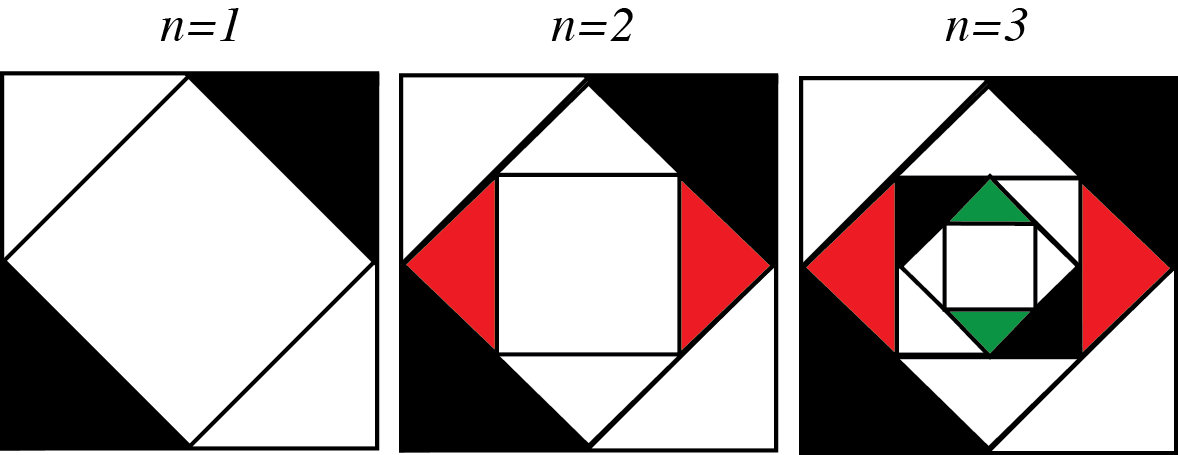
\includegraphics{Images/squares-diagram.png}
        \caption{Different Iterations of the fractal}
        \label{squares-diagram}
    \end{figure}
    \begin{knowledge}
        \item Geometric series with a fixed amount of terms.
        \item Geometric series with an infinite amount of terms.
    \end{knowledge}
    \subquestion{What is the total area of the saded region if the process is continued for a total of 10 iterations?}
    \begin{solns}
        \step{Setting the problem up}
        What can be helpful in this situation is to create a table for each of the iterations of the fractal, and to do some calculations on the side:\par
        \vspace{0.5cm}
        \substep{calculations for $n=1$}
            Divide the square into 8 triangular sections as shown in Figure \ref{square-n-1}.
            \begin{figure}[H]
                \centering
                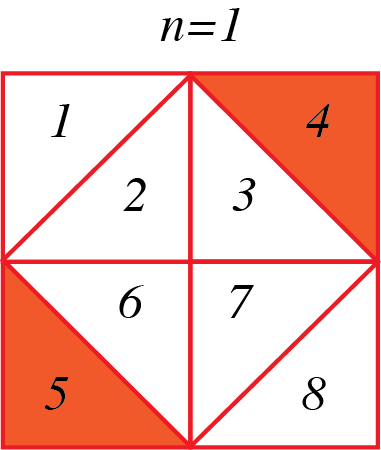
\includegraphics{Images/square-n-1.png}
                \caption{Diving the square into several sections}
                \label{square-n-1}
            \end{figure}
            Notice $\frac{2}{8}$, or $\frac{1}{4}$ of these triangular sections are shaded. This means that $\frac{1}{4}$ of the area of the square is shaded, as shown in Table \ref{shaded-regions}.
            \substep{calculations for $n=2$}
            Each section's hypotenuse is the side length of the newly iterated square, as shown in Figure \ref{one-section}.
            \begin{figure}[H]
                \centering
                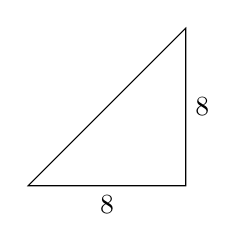
\begin{tikzpicture}
                    \draw {(0,0) -- node[anchor=north] {8} (2,0) -- node[anchor=west] {8} (2,2) -- cycle};
                \end{tikzpicture}
                \caption{One section}
                \label{one-section}
            \end{figure}
            \begin{solnstable}
                $c = \sqrt{8^2 + 8^2}$ & By Pythagorean Theorem \\
                $c = 8\sqrt{2}$ & \\
            \end{solnstable}
            The total area of the smaller rectangle is therefore $\left(8\sqrt{2}\right)^2$, and the shaded region is one quarter of that area, as shown in Table \ref{shaded-regions}.
            \substep{calculations for $n=3$}
            Here, we repeat the same calculations, but with a smaller value of $\frac{8\sqrt{2}}{2}$ instead of $\frac{16}{2}$.
            \begin{figure}[H]
                \centering
                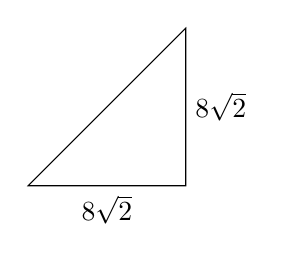
\begin{tikzpicture}
                    \draw {(0,0) -- node[anchor=north] {$8\sqrt{2}$} (2,0) -- node[anchor=west] {$8\sqrt{2}$} (2,2) -- cycle};
                \end{tikzpicture}
                \caption{A smaller section}
            \end{figure}
            \textbf{Note:}\space The \emph{shaded region} cell is not the compounded area. It does not take into consideration previous iterations.
            \begin{table}[H]
                \centering
                \renewcommand{\arraystretch}{1.5}
                \begin{tabular}{c|c}
                    $n$ & Shaded Region \\
                    \hline
                    1 & $\frac{1}{4} \cdot 256 = 64$ \\
                    \hline
                    2 & $\frac{1}{4} \cdot 128 = 32$ \\
                    \hline
                    3 & $\frac{1}{4} \cdot 64 = 16$ \\
                    \hline
                \end{tabular}
                \caption{Calculating the areas of the shaded regions}
                \label{shaded-regions}
            \end{table}
            Notice how each area is essentially the previous divided by two. This is a geometric sequence with $a_0 = 64$ and $r = \frac{1}{2}$.
        \step{Solving for the sum of a geometric sequence}
        \begin{solnstable}
            $S_n = a_0\frac{1-r^n}{1-r}$ & Use the formula for a geometric series with $n$ terms. \\
            $S_10 = 64\frac{1-r^{\frac{1}{4}}}{1-\frac{1}{4}}$ & Plug all values in \\
            $S_10 = 127.875$ & \\
        \end{solnstable}
        \begin{answer}
            $S_10 = 127.875$
        \end{answer}
    \end{solns}
    \subquestion{Suppose this process were to contiue on forever. What would be the total shaded area?}
    \begin{solns}
        \step{Solving for an infinite geometric series}
        \begin{solnstable}
            $S_{\text{inf}} = a_0\frac{1}{1-r}$ & The sum of an infinite geometric series \\
            $S_{\text{ing}} = 64\frac{1}{1-\frac{1}{2}}$ & Sub in all the values \\
        \end{solnstable}
        \begin{answer}
            $S_{\text{inf}} = 128$
        \end{answer}
    \end{solns}
    \section{Mathematical Induction}
    \question{Prove the following statements using mathematical induction $\forall n \in \mathbb{Z}^{\star}$}
    \begin{knowledge}
        \item Mathematical induction with equalities
        \item Mathematical induction with inequalities
    \end{knowledge}
    \begin{solns}
        \step{Define the statement}
        $$
            p(n): \sum_{i=1}^{n}\left(i\frac{1}{2}\right)^{i-1} = 4 - \frac{n+2}{2^{n-1}}; \forall n \in \mathbb{Z}^{\star}
        $$
        \step{Prove it holds true for a certain base case}
        \begin{solnstable}
            $p(1): 1 = 4 - \frac{1+2}{2^{1-1}}$ & Plug 1 into $p(x)$ \\
            $1 = 4 -3 $ & \\
            $1 = 1$ & Simplify \\  
        \end{solnstable}
        \step{Assume $p(k)$ is true}
        $$
            p(x): \sum_{i=1}^{k}i\left(\frac{1}{2}\right)^{i-1} = 4 - \frac{k + 2}{2^{k-1}}; \forall k \in \mathbb{Z}^{\star}
        $$
        \step{Prove $p(k+1)$ is true}
        \begin{solnstable}
            $p(k+1): \sum_{i=0}^{k+1}i\left(\frac{1}{2}\right)^{i-1} = 4 - \frac{k + 3}{2^k}$ & State $p(k+1)$ \\
            $LS = \sum_{i=1}^{k}i\left(\frac{1}{2}\right)^{i-1}+\left(k+1\right)\left(\frac{1}{2}\right)^{k} = 4$ & Start by looking at the left side. Split the summation. \\
            $LS = 4-\frac{k+1}{2^{k-1}}+\frac{k+1}{2^k}$ & Replace $\sum_{i=1}^{k}i\left(\frac{1}{2}\right)^{i-1}$ with $p(k)$. \\
            $LS = 4 + \frac{2(k-2)+k+1}{2^k}$ & Combine with a common denominator of $2^k$, by multiplying $\frac{k+2}{2^{k-1}}$ by 2 as $2^{k+1} \cdot 2 = 2^k$. \\
            $LS = 4 + \frac{-2k - 4 + k + 1}{2^k}$ & \\
            $LS = 4+\frac{-k-3}{2^k}$ & \\
            $LS = 4-\frac{k+3}{2^k} = RS$ & The left side equals the right side after some simplification. \\
        \end{solnstable}
        \step{Conclusion}
        By the principle of mathematical induction, $p(x)$ is true.
    \end{solns}
    \subquestion{$(1-a)^n > 1-na$, where $n \geq 2$, $0 < a < 1$}
    \begin{solns}
        \step{Define the statement}
        $$
            p(n): (1-a)^n > 1-na; \space\forall n \in \mathbb{N},\space n \geq 2, \space 0 < a < 1
        $$
        \step{Prove $p(n)$ holds for the smallest possible value}
        \begin{solnstable}
            $p(2):\space (1-a)^2 > 1-2a$ & The smallest possible value in this problem, according to the question, is not one but two. Plug this value in $p(n)$. \\
            $1-2a+a^2 > 1-2a$ & This is true so long as $a>0$, as adding something to the same value will will make it bigger. For instance, suppose $1-2a$ is -1 (so $a=1$). $-1+a^2$ would be greater than $-1$, so long as $a > 0$.
        \end{solnstable}
        \step{Assume $p(k)$ is true}
        $$
            p(k): (1-a)^k > 1-ka;\space\forall k \in\mathbb{N}^{\star}
        $$
        \step{Prove $p(k+1)$ is true}
        $$
            p(k+1): (1-a)^{k+1} \stackrel{?}{>} 1-(k+1)a
        $$
        \begin{solnstable}
            $\text{LS} = (1-a)^{k+1}$ & \\
            $= (1-a)^k(1-a)$ & Expand the term so that $p(k)$ can be substituted into the inequality. \\
            $=(1-ka)(1-a)$ & Substitute $1-ka$ for $(1-a)^k$. \\
            $= 1 -a -ka +ka^2$ & \\
            $= 1-(k+1)a + ka^2$ & Simplify and rearrange \\
            $1-(k+1)a + ka^2 > 1-(k+1)a $ & This is true as $ka^2$ is being added to essentially the same term on the right side. So long as $a>0$, this holds.
        \end{solnstable}
        \step{Conclusion}
        By the principle of mathematical induction, $p(n)$ is true.
    \end{solns}
    \section{Quadratic Functions}
    \question{Solve for $x$ in equation $x^2 - (a+3b)x + 3ab = 0$ (note that $x$ is in terms of $a$ and $b$)}
    \begin{knowledge}
        \item Quadratic formula
    \end{knowledge}
    \begin{solns}
        \begin{solnstable}
            $x^2 - (a+3b)x + 3ab = 0$ & State the equation \\
            $ax^2 + bx + c$ & The general form of a quadratic function \\
            $a = 1$ & \\
            $b = -(a+3b)$ & \\
            $c = 3ab$ & \\
            $x = \frac{-b \pm\sqrt{b^2 -4ac}}{2c}$ & The quadratic formula \\
            $= \frac{-(-(a+3b))\pm\sqrt{(a+3b)^2 - 4(1)(3ab)}}{2}$ & Plug in all values \\
            $= \frac{a+3b \pm \sqrt{a^2 + 6ab + 9b^2 -12ab}}{2}$ \\
            $= \frac{a+3b \pm \sqrt{a^2 - 6 ab + 9b^2}}{2}$ \\
            $= \frac{a+3b \pm \sqrt{(a-3b)^2}}{2}$ \\
            $x = \frac{a+3b \pm (a-3b)}{2}$ & Some simplification... \\
            $x = a$ \\
            $x = 3b$ \\
        \end{solnstable}
        \begin{answer}
            $x \in \left\{a, 3b\right\}$
        \end{answer}
    \end{solns}
    \question{Find the value of $c$ such that the vertex of the below paraboa is $\left(\frac{4}{3},\frac{-1}{3}\right)$:
    $$
        3x^2 - 8 x + c
    $$
    }
    \begin{knowledge}
        \item Formulae for $n$ and $k$ of the vertex of a parabola.
    \end{knowledge}
    \begin{solns}
        \step{State what is known}
        $a=3$ \\
        $b=-8$ \\
        $c=c$ \\
        \step{Calculate the $k$ of the parabola}
        \begin{solnstable}
            $k=\frac{-\Delta}{4a}$ & Formula for $k$ \\
            $=\frac{4ac-b^2}{4a}$ & \\
            $=\frac{4(3)c-(-8)^2}{4(3)}$ & \\
            $=\frac{12c-64}{12}$ & \\
            $=\frac{3c-16}{3}$ & Simplify
        \end{solnstable}
        \step{Solve for $c$}
        \begin{solnstable}
            $\frac{3c-16}{3} = \frac{-1}{3}$ & Equate the formula for the $k$ value in terms of $c$ to the formula given in the question. \\
            $3c-16 = -1$ & \\
            $c=5$ & Simplify \\
        \end{solnstable}
        \begin{answer}
            $c=5$
        \end{answer}
        \begin{checkanswer}
            There is an alternate way of solving for $k$, which is of doing $f(h)$.
            \mdfsubtitle{Calculate $h$ of the parabola}
            \begin{solnstable}
                $h=\frac{-b}{2a}$ & The formula for $h$. \\
                $\frac{4}{3}$ & Simplify \\
            \end{solnstable}
            \mdfsubtitle{Find $k$ in terms of $c$}
            \begin{solnstable}
                $f\left(\frac{4}{3}\right)=\frac{-1}{3}$ & Plug $h$ into the function to find the corresponding $y$ value \\
                $3\left(\frac{4}{3}\right)^{2}-8\left(\frac{4}{3}\right)+c$ & Expand \\
                $\frac{16}{3}-\frac{32}{3}+c$ \\
                $\frac{-16}{3}+c$ \\
            \end{solnstable}
            \mdfsubtitle{Equate the value of $k$ in terms of $c$ with the value given in the question.}
            \textbf{Note:}\space Although we could keep on going here, it is not necessary, as we know that the value of $k$ we have obtained is identical to the one we got via the other method.
            $$
                \frac{3c-16}{3} = c-\frac{16}{3}
            $$
        \end{checkanswer}
    \end{solns}
    \question{The quadratic function $f(x)$ has the following properties:
        \begin{enumerate}
            \item It passes through point (2,4)
            \item It has a maximum value of 6 when $x=4$
            \item It has a zero of $x=-4+2\sqrt{3}$
        \end{enumerate}
        If the function is of the form $ax^2+bx+c$, find the values of $a$, $b$, and $c$.}
        \begin{knowledge}
            \item Vertex form of a parabola
            \item Expanding vertex form into general form
        \end{knowledge}
        \begin{solns}
            \step{Find the Vertex Form}
            \begin{solnstable}
                $f(x)=a(x-h)^2+k$ & The generalized vertex form of a parabola. \\
                $=a(x-4)^2 + 6$ & It is said in the question, albeit with different wording, that the vertex of the parabola is at $(4,6)$. \\
                $4 = a(2-a)^2 + 6$ & It is said that the parabola passes through point $(2,4)$ \\
                $4 = 4a + 6$ & \\
                $-2 = 4a$ & \\
                $a = \frac{-1}{2}$ \\ 
            \end{solnstable}
            \step{Expand Vertex Form into Standard Form}
            \begin{solnstable}
                $\frac{-1}{2}(x-4)^2 + 6$ & The vertex form from the previous step \\
                $\frac{-1}{2}(x^2 - 8x + 16) + 6$ \\
                $\frac{-1}{2}x^2 + 4x -2$ & Simplify \\
            \end{solnstable}
            \begin{answer}
                $a = \frac{-1}{2}$ \\
                $b = 4$ \\
                $c = -2$ \\
            \end{answer}
            \begin{checkanswer}
                To solve this problem, we did not need to know the third piece of information that was given to us. That said, knowing one of the roots does help us check our answers.
                \mdfsubtitle{Find Roots of The Polynomial}
                \begin{solnstable}
                    $\frac{-1}{2}x^2 + 4x -2 = 0$ & Our polynomial from before \\
                    $x=-4 \pm \sqrt{12}$ & These are both roots \\
                    $x \in \left\{ -4-\sqrt{12},-4+\sqrt{12} \right\{$
                \end{solnstable}
                The root $-4+\sqrt{12}$ corresponds to the root that was given to us, being $-4+2\sqrt{3}$
            \end{checkanswer}
        \end{solns}
    \question{Consider the function $p(x) = mx^2 -2(m+2)x+m+2$}
    \subquestion{Find all values $m$ such that $p(x)$ has two real roots.}
    \begin{solns}
        This is a discriminant question, as it asks for the \emph{number} of roots.
        \begin{solnstable}
            $\Delta \geq 0$ & For $p(x)$ to have two real roots, its discriminate must be greater than or equal to 0. The question never says it can't be the same zero twice. \\
            $b^2 - 4ac \geq 0$ & Expand $\Delta$ \\
            $(-2m-4)^2 -4(m)(m+2) \geq 0$ & Plug in the proper values \\
            $4m^2 +16m +16 -4m^2 -8m \geq 0$ & \\
            $8m + 16 > 0$ & \\
            $m > -2$ & Simplify... \\
        \end{solnstable}
        \begin{answer}
            $m > 2;~m \neq 0$
        \end{answer}
        \begin{checkanswer}
            To check the answer, we test for a value of $m$ less than 2, a value of $m$ equal to 2, and a value of $m$ greater than 2.
            \mdfsubtitle{$m=-3$}
            \begin{solnstable}
                $mx^2 -2(m+2)x + m + 2 = 0$ & State the question \\
                $-3x^2 -2(-1)x -1 = 0$ & Plug in $m=-3$. \\
                $-3x^2 +2x -1 = 0$ & Simplify \\
                $\Delta = (-3)^2 -4(-3)(-1)$ & State the discriminant \\
                $\Delta = -3$ & Simplify. \\
            \end{solnstable}
            $m$ has no roots at $m=-3$
            \mdfsubtitle{$m=-2$}
            \begin{solnstable}
                $mx^2 -2(m+2)x + m + 2 = 0$ & State the question \\
                $-2x^2$ & Plug in $m=-2$ \\
                $\Delta = 0-4(-2)(0)$ & Find the discriminant \\
            \end{solnstable}
            $m$ has one root ($\sqrt{0}$) at $m=-2$.
            \mdfsubtitle{$m=-1$}
            \begin{solnstable}
                $mx^2 -2(m+2)x + m + 2 = 0$ & State the question \\
                $-x^2 -2(1)x -1 + 2 = 0$ & Substitute $-1$ as the value of $m$. \\
                $-x^2 -2x +1 = 0$ & Simplify \\
                $\Delta = 4-4(-1)(1)$ & Find the discriminant \\
            \end{solnstable}
            $m$ has more than one root at $m=-1$
        \end{checkanswer}
    \end{solns}
    \subquestion{Has two positive roots.}
    \begin{solns}
        \step{Find the roots of $m$}
        \begin{solnstable}
            $x=\frac{-b\pm\sqrt{b^2-4ac}}{2a}$ & The quadratic formula represents both roots \\
            $a = m,~b = -2(m+2),~ c=m+2$ & State $a$, $b$, and $c$. \\
            $x=\frac{2m+4\pm\sqrt{4m^2 + 16m + 16 -4(m)(m+2)}}{2m}$ & Plug in $a$, $b$, and $c$. \\

        \end{solnstable}
    \end{solns}
    \subquestion{Has one positive and one negative root.}
    \section{Linear Inequalities}
    \question{What values of $x$ solve the following inequality?
    $$
        \frac{3x-2}{5} + 3 \geq \frac{4x-1}{3}
    $$
    }
    \begin{solns}
        \begin{solnstable}
            $\frac{3x-2+15}{5} \geq \frac{4x-1}{3}$ & \\
            $\frac{3x+13}{5} \geq \frac{4x-1}{3}$ & Combine the left side under a common denominator of 5. \\ 
            $15 \cdot \frac{3x+15}{5} \geq \frac{4x-1}{3} \cdot 15$ & Multiply both sides by 15, as it is the $lcm(5, 3)$. The inequality remains unchanged as these values are both greater than 0. \\
            $9x+39 \geq 20x-5$ & \\
            $44 \geq 11x$ & \\
            $4 \geq x$ & \\
            $x \leq 4$ & Some simplification allows us to get the solution.
        \end{solnstable}
        \begin{answer}
            $x \leq 4$
        \end{answer}
        \begin{checkanswer}
            \mdfsubtitle{Check at 4}
            \begin{solnstable}
                $\frac{3(4)-2}{5} + 3 \geq?  \frac{4(4)-1}{3}$ & Plug 4 as $x$. \\
                $5 \geq? 5$ & Simplify.
            \end{solnstable}
            \TRUE at 4\space\checkmark
            \mdfsubtitle{Check at 3}
            \begin{solnstable}
                $\frac{3(3)-2}{5} + 3 \geq?  \frac{4(3)-1}{3}$ & Plug 3 as $x$ \\
                $\frac{22}{5} \geq? \frac{11}{3}$ & Simplify ... \\
                $\frac{66}{15} \geq? \frac{55}{15}$ & Common denominator \\
            \end{solnstable}
            \TRUE at 3\space\checkmark
            \mdfsubtitle{Check 5}
            \begin{solnstable}
                $\frac{3(5)-2}{5} + 3 \geq? \frac{4(5)-1}{3}$ & Plug 5 in as $x$ \\
                $\frac{28}{5} \geq? \frac{19}{3}$ & Simplify \\
                $\frac{84}{15} \geq? \frac{95}{15}$ & Common denominator \\
            \end{solnstable}
            \FALSE at 5\space\checkmark\par
        \end{checkanswer}
    \end{solns}
\end{document}